

\documentclass{article}

\usepackage{amsmath}
\usepackage{graphicx}
\usepackage{float}
\usepackage{natbib}
\bibliographystyle{apalike}
\usepackage[nottoc]{tocbibind}
\usepackage{appendix}
\usepackage{listings}


\author{Qing Scholten, Wessel van Sommeren}
\title{Controlling a rabbit plaque}

\begin{document}

\maketitle
\newpage
\tableofcontents
\newpage

\section{Introduction}
In 1859 the First Fleet of settlers arrived in Australia, with them Thomas Austin. Thomas Austin took 13 European rabbits with him on his journey, so that once in Australia he could set them free so that he could hunt them for food. What Thomas Austin did not know was that these European rabbits did not have any natural predators or competition in australia. So by 1920 the small population of 13 rabbits had turned into a rabbit plaque, in 1920 there were an estimated 10 billion rabbits in australia.In this paper we will attempt to model the rabbit plaque of australia by exploring the question "What is the most effective way to control a rabbit plaque comparing Hunting and Introducing predators?".
\section{Rabbit population growth}
For the base case we use the fact that a rabbit on average gets 4 - 8 babies per 60 days. So we take 6 on average that means one rabbit produces 0.1 rabbit per day. A rabbit in the wild live up to 9 nine years this means 0.000312109862672 rabbits die per day per rabbit. This means we get 
$$
\frac{dP(t)}{dt} = 0.1P(t)-0.000312109862672P(t)
$$

We take $P(0) = 13$ as starting population
\\

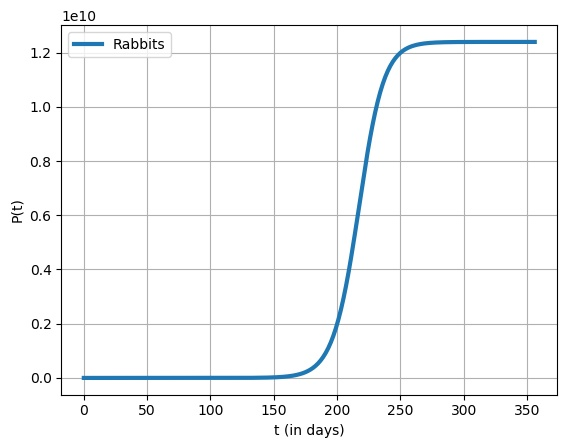
\includegraphics[scale=0.78]{Pictures/unr_rabbitts}
\\ 
As we can see from the graph de population of 13 rabbits grew to more than  $2.5\cdot10^{11}$ in just 250 days. This would continue to grow exponentially forever as the current model does not have a limiting factor. The limiting factor in our model is going to be food. As Australia has about 7 616 666 square kilometer land and 1 371 000 square kilometer of this land is desert, one finds that about 7 479 566 square kilometer is fertile land. This follows from the assumption that every land outside the deserts is able to grow grass, which is the vegetation that is used in the model. Known is that "the average annual total herbage production at Moorepark for the period 2005–9 was 14 087 kg DM/ ha, with an average grass growth of 50·3 kg DM/ha/day." A 1 hectare is equal to 0.01 square kilometer, the avarage annual total herbage production 140.87 kg $Dm/km^2$, so for Australia this is about 1 052 646 462 kg Dm. This means that the amount of grass, as grass has about 17 dry material, is about 6 197 920 367 kg grass for the whole of Australia. As rabbits eat around 1 cup of grass for 2 lbs of body weight, this would convert to about 0.25 kilo gram grass for a medium sized rabbit of 2 kilo gram. This means that Australia has enough grass to house 12 395 840 734 rabbits without running out of food.

Let $R$ be the reproduction number
$$
R = 0.1 - 0.000312109862672
$$
$$
\frac{dP(t)}{dt} = RP(t)(1-\frac{P}{12 395 840 734})
$$
\\
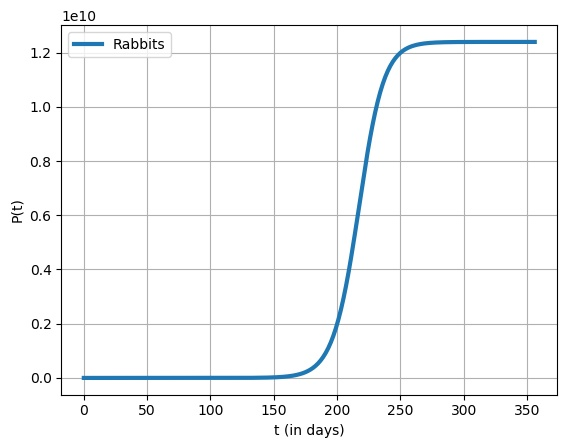
\includegraphics[scale=0.78]{Pictures/logis}
\\

From the graph we see that the model reaches an equilibrium around 12 395 840 734, which is what we expected and wanted. This can also be confirmed analytically 
$$
0= RP(t)(1-\frac{P(t)}{12 395 840 734})
$$
$$
RP(t) = 0
$$
$$
1-\frac{P(t)}{12 395 840 734} = 0
$$
$$
P(t) = 12 395 840 734
$$
This shows that the equilibrium solutions are 0 and 12 395 840 734
$$
M = 12 395 840 734 
$$
$$
\frac{dP(t)}{dt} = RP(t)(1 - \frac{1}{M}P(t))
$$
$$
\frac{dP(t)}{P(t)(1 - \frac{1}{M}P(t))} = Rdt
$$
$$
\frac{MdP(t)}{P(t)(M - P(t))} = Rdt
$$
$$
dP(t)(\frac{-1}{P(t)} - \frac{1}{M -P(t)})   = Rdt
$$
$$
\int{(\frac{1}{P(t)} - \frac{-1}{M -P(t)})dP(t) }  =\int{ R}dt
$$
$$
\ln(P(t)) - \ln(M -P(t)) + c_1 = Rt +c_2
$$

$$
 \ln(\frac{P(t)}{M -P(t)})  = Rt +c
$$

$$
\frac{P(t)}{M -P(t)}= e^{Rt +c}
$$

$$
P(t) = - \frac{Me^{Rt +c}}{1 - e^{Rt +c}}
$$
$$
P(0)(1 - e^{c}) = -Me^{c}
$$
$$
c = \ln(\frac{P(0)}{P(0)-M})
$$
$$
P(t) =  \frac{MP(0)}{P(0)+(M - P(0))e^{-Rt}}
$$
\section{Hunting}
First we will explore one of the most obvious solutions to a plaque of animals. Hunting animals might be an obvious solution however we will look at how sustainable this solution is in the long term since introducing hunters does not actually impact the carrying capacity of an ecosystem. To model this we start at the base case 
$$
\frac{dP(t)}{dt} = RP(t)(1-\frac{P(t)}{M})
$$
expanded this looks like 
$$
\frac{dP(t)}{dt} = RP(t)-\frac{RP^2(t)}{M}
$$
we need to add an extra negative term for the hunters. The amount of hunters would be proportional to the size of the population of the rabbits
$$
H(t) = C_1 P(t)
$$
Where H is the amount of hunters and $C_1$ is a constant. Those hunters will impact the population of rabbits so a hunter term is added to the base case
$$
\frac{dP(t)}{dt} = RP(t)-\frac{RP^2(t)}{M} - \beta H(t)
$$
$\beta$ is the amount representing the amount 1 hunter can kill per day. However since we know $H(t)$ we can re substitute this back into the equation
$$
\frac{dP(t)}{dt} = RP(t)-\frac{RP^2(t)}{M} - \beta C_1 P(t)
$$
$\beta $ is also depended on the population of rabbits, since its easier to find and kill a rabbit if there are a lot per square kilometer. Therefore beta is proportional to population of rabbits per square kilometer
$$
\beta = C_2 \frac{P(t)}{A}
$$

$$A = \text{The area of australia}$$
Substituting this will get 
$$
\frac{dP(t)}{dt} = RP(t)-\frac{RP^2(t)}{M} - C_2 C_1 \frac{P^2(t)}{A}
$$

Lets assume a hunter can cover a area of 10 square kilometers per day and is $50\%$ effective then $C_2 = 5$. For  $C_1$ we can use the equilibrium to determine a suitable constant. 
$$RP(t)-\frac{RP^2(t)}{M} - C_2 C_1 \frac{P^2(t)}{A} = 0$$
$$ R-\frac{RP(t)}{M} - C_2 C_1 \frac{P(t)}{A} = 0, P = 0 $$
$$ C_1 = \frac{R-\frac{RP(t)}{M}}{C_2 \frac{P(t)}{A}} $$

Now we can choose a population of rabbits that we deem apporopiate and find $C_1$
\\
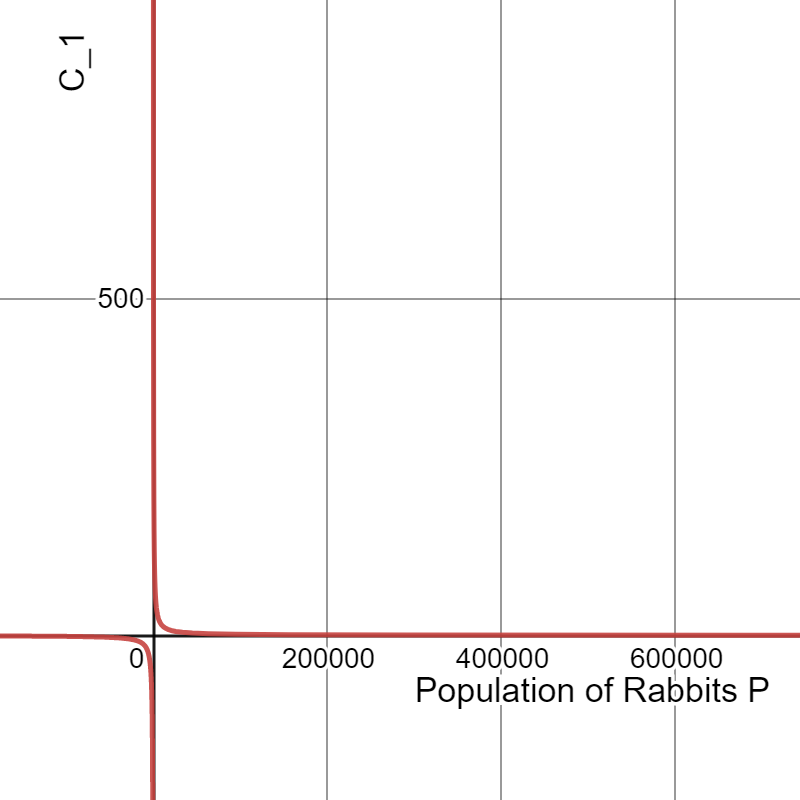
\includegraphics[scale=0.4]{Pictures/C_1-P}
\\
The amount of hunters was determined by 
$$H(t) = C_1 P(t)$$
$$ C_1 = \frac{R-\frac{RP(t)}{M}}{C_2 \frac{P(t)}{A}} $$
$$H=\frac{R-\frac{RP}{M}}{C_2 \frac{P}{A}}P$$
$$H = A\frac{R-\frac{RP}{M}}{C_2}$$
\\
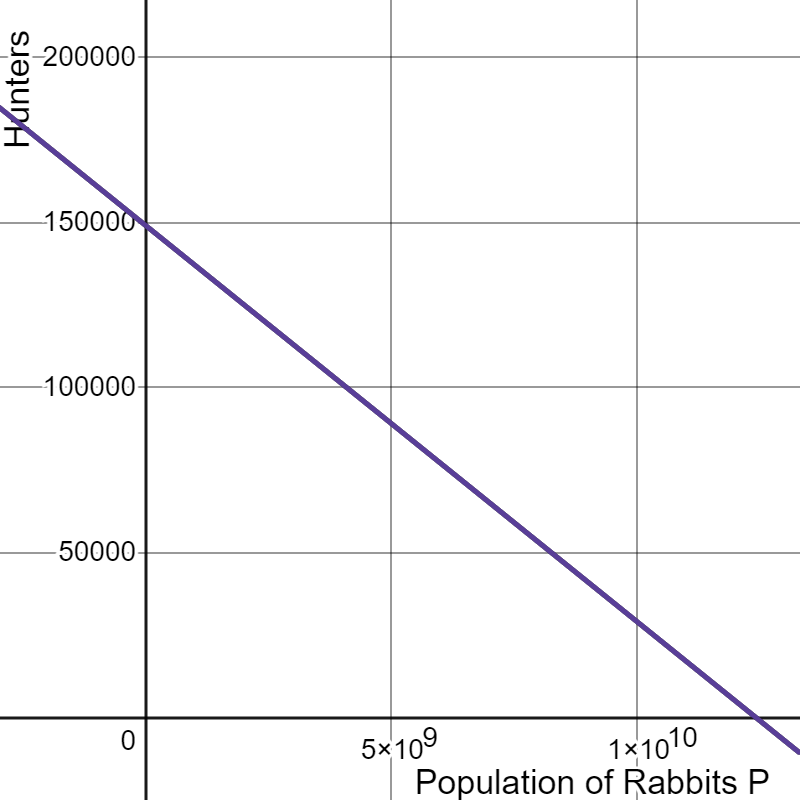
\includegraphics[scale=0.3]{Pictures/H-P}
\\
From this graph we can see that if we want for example an equilibrium of 1000 rabbits we would pick $C_1 = 149.124418706$ which would mean we would need to hire 149124.418706 hunters and if we use eulers method to solve for P we would indeed find that this is correct
\\
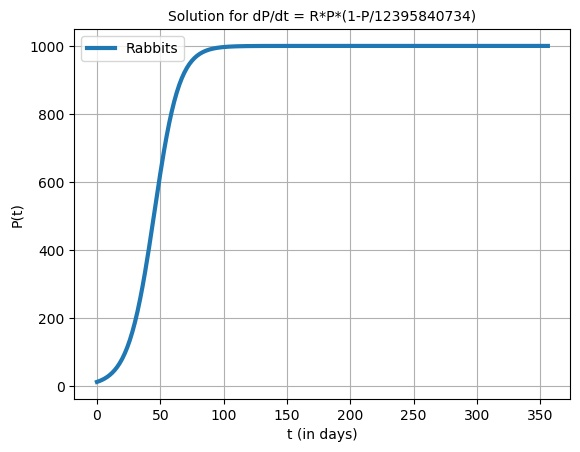
\includegraphics[scale=0.5]{Pictures/1000H}
\\
However this is not realistic for two main reasons. First of all the population is highly unstable because if we pick $C_1 = 14.9124310435$ because we want a population of 10000 we would need to hire 149124.310435 hunters to keep te population stable which is only 0.108271790959 more hunters than for a stable population if 1000 Secondly it does not make sense for a goverment to hire that much hunters to keep a population that low. It would mean by far the most of them would be doing nothing per day.
\\
The amount of rabbits killed per hunter per day is the base case at the equilibrium P devided by the amount of hunters at equilibrium P So
$$\frac{RP(1-\frac{P}{M})}{H}$$
One wild rabbit can be sold for approximatially 15 euro and a hunter makes about 35000 euro per year. So if the hunter can sell a lot of rabbits it will be cheaper for the goverment since they would not have to subsidize those hunters as much. 
$$\text{cost} = H(35000 -15\beta) $$
$$\text{cost} = A\frac{R-\frac{RP}{M}}{C_2}(35000  -15C_2 \frac{P}{A}) $$
\\
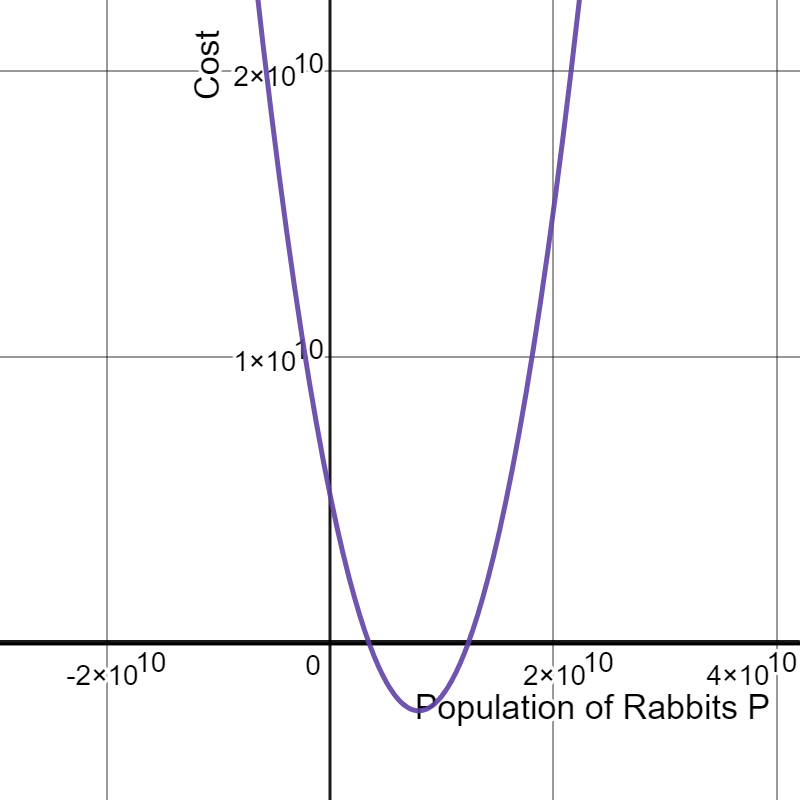
\includegraphics[scale=0.3]{Pictures/CostH}
\\



\section{Introducing a predator: The Red Fox}
Australia 7 616 666 square kilometer land, of which 1 371 000 square kilometer is desert. Knowing that red foxes don't live in the desert, they have about 7 479 566 square kilometer land to live on. The red fox has a territory that ranges one to two miles from its home. Assuming that the territory of a red fox is circular with a radius of one mile, this means that the area a red fox needs is $\pi*1^2$ which is equal to about 3.14 square mile per fox.\cite{FoxTerritoryReproduction} Converting this to square kilometer, the fox needs about 8.13 square kilometer of space. This means that Australia can house about 919 996 red foxes, without getting overcrowded. As foxes reproduce every 51 days and get on average 5 pups per two foxes, meaning that every fox wil get 2.5 pups in 51 days on average.\cite{FoxTerritoryReproduction} This means that the birth rate is about 0.0245 pups per fox per day. Red foxes live nine years on average.\cite{FoxLife} This means that the death rate is about 0.0003044 deaths per fox per day.

Let $R_f$ be the reproduction number.
$$R_f = b_f - d_f$$
$$b_f = 0.0245$$
$$d_f = 0.0003044$$
$$\frac{dP_f(t)}{dt} = R_fP_f(t)(1-\frac{P_f(t)}{M_f})$$
$$M_f = 919996$$
\begin{figure}[h!]
    \centering
    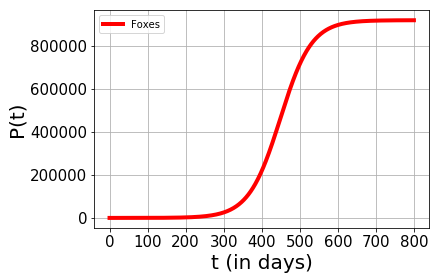
\includegraphics[scale=0.78]{Pictures/Foxes.png}
    \caption{Solution for $\frac{dP_f(t)}{dt} = R_fP_f(t)(1-\frac{P_f(t)}{M_f})$ where the foxes start at $20$}
    \label{fig:Foxes}
\end{figure}
From Figure \ref{fig:Foxes} we see that the model reaches an equilibrium around 919996, which is expected and wanted. This can also be confirmed analytically.
$$0=R_fP_f(t)(1-\frac{P_f(t)}{M_f})$$
$$R_fP_f(t)=0$$
$$1-\frac{P_f(t)}{M_f}=0$$
$$P_f(t)=M_f$$
$$P_f(t)=919996$$
This shows that the equilibrium solutions are 0 and 919996. In an equilibrium situation, the extra deathrate due to lack of space can be found by the following formula, as the extra deathrate is dependent on both the maximum amount of foxes and the growth rate of the amount of foxes.
$$\alpha_f = a_f * \overline{F}$$
Where $\alpha_f$ is $b_f-d_f$, $a_f$ is the extra deathrate on top of the constant deathrate due to space limitations and $\overline{F}$ is the amount of foxes in the equilibrium situation where
$$\overline{F} = 919996$$
This means that we can find the $a_f$ with the following formula
$$a_f = \frac{\alpha_f}{\overline{F}}$$
With this can be found that $a_f = 0.000000063$. The extra birthrate dependent on the amount of food (namely rabbits) available can be found by
$$\alpha_f + c_f*\overline{K}-a_f*\overline{F}=0$$
As the extra birthrate should be depend on the amount of rabbits, amount of foxes, the extra deathrate and the growth rate of the foxes, where $c_f$ is the extra birthrate dependent on the amount of food and $\overline{K}$ is the amount of rabbits in the equilibrium situation where
$$\overline{K}=12395840734$$
This means that we can find $c_f$ with the following formula
$$c_f=\frac{-\alpha_f+a_f*\overline{F}}{\overline{K}}$$
$$c_f=\frac{-\alpha_f+\frac{\alpha}{\overline{F}}*\overline{F}}{\overline{K}}$$
So we find that $c_f=0$. This means that the differential equation becomes 
$$\frac{dP_f(t)}{dt}=(b_f-d_f)*P_f*(1-\frac{P_f}{M_f})$$
We find that, as red foxes eat around 500 grams of food per day, a red fox eats about 0.25 rabbits a day when available, but their diet is dependent on how easy accessible the rabbits are, so more rabbits, means it's easier for the foxes to eat he rabbits.\cite{FoxFood} We find the extra deathrate due to foxes with the following formula, as this is dependent on the amount of foxes and the amount of rabbits.
$$a_k*\overline{F}*\overline{K}=0.25*\overline{F}$$
So we find now that we can find the extra deaths of rabbits due to foxes with
$$a_k=\frac{0.25}{\overline{K}}$$
Which means that $a_k=2.0168*10^{-11}$. This means we have the following derivative equations
$$\frac{dP_k}{dt}=(b_k-d_k)*P_k*(1-\frac{P_k}{M_k})-a_k*P_k*P_f$$
and
$$\frac{dP_f}{dt}=(b_f-d_f)*P_f*(1-\frac{P_f}{M_f})$$
\begin{figure}[ht!]
    \centering
    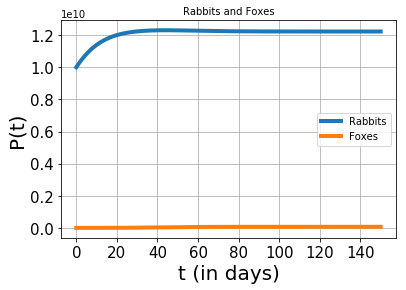
\includegraphics[scale=0.78]{Pictures/RabbitFoxes.png}
    \caption{Solutions for $\frac{dP_k}{dt}=(b_k-d_k)*P_k*(1-\frac{P_k}{M_k})-a_k*P_k*P_f$ and $\frac{dP_f}{dt}=(b_f-d_f)*P_f*(1-\frac{P_f}{M_f})$, where the rabbits start at $10*10^{10}$ and the foxes start at $919996$}
    \label{fig:RabbitFoxes}
\end{figure}
In Figure \ref{fig:RabbitFoxes} the situation is plotted where there are 10000000000 rabbits and 919996 foxes, which is about the amount of rabbits Australia has when they had their big rabbit plague and the maximum amount of foxes that can live in Australia. In the graph one can see that due to the low maximum amount of foxes that can live in Australia, they don't do much to the rabbits, where they grow their amount to the equilibrium of $1.23935344*10^10$. The foxes have their equilibrium around $919996$. As the foxes only eat around 0.25 rabbit per fox at the most, they don't do much as a relatively small number of foxes can be housed in Australia in comparison to the amount of rabbits. The code for this model can be found in appendix \ref{FoxRabbitModel}.
%https://cosleyzoo.org/red-fox/#:~:text=Shelter%20and%20Space%20Needs&text=The%20normal%20territory%20of%20the,remarkably%20to%20cohabitation%20with%20humans.
%https://ofnc.ca/programs/fletcher-wildlife-garden/flora-and-fauna-at-the-fwg/red-foxes-at-the-fwg
%https://www.nhm.ac.uk/discover/the-secret-life-of-urban-foxes.html#:~:text=Wild%20red%20foxes%20generally%20live,between%20one%20and%20three%20years.
%https://www.wildlifeonline.me.uk/animals/article/red-fox-diet-how-much-food#:~:text=Again%2C%20this%20is%20a%20deceptively,pound)%20of%20food%20per%20day.
%https://ofnc.ca/programs/fletcher-wildlife-garden/flora-and-fauna-at-the-fwg/red-foxes-at-the-fwg
\section{Introducing a predator: The Grey Wolf}
Knowing that red foxes take up to much space for the amount of rabbits they eat, introducing another predator instead of red foxes, that live in groups on a territory and eat more rabbits per day, may work. In this case we look at wolves, as they live in packs and eat around ten times as much as a red fox. Grey wolves need to eat about five to seven pounds per wolf per day, as we assume they reproduce constantly.\cite{WolfFood} This means they eat 2.26796 to 3.17515 kilogram per day per wolf. Using the average of this, we get that a wolf eats 2.721555 kilogram a day. As we use rabbits of around 2 kilograms, a wolf eats around 1.3607775 rabbit a day in the optimal circumstances. As grey wolves have a gestation period of on average 63 days  and they have 4 to 6 pups on average, the birth rate on average is about 0.03968 pups per day per wolf.\cite{WolfRepLifeTer} As the territory of a pack, which is on average consisting of 7 wolves, is around 70 to 700 square miles.\cite{WolfRepLifeTer} As we want as much wolves as possible on the continent of Australia, we use 70 square miles, or about 181.3 for a pack of 7 wolves. This means that with around 7 479 566 square kilometer of land to live on, since wolves don't live in deserts, there is space for 41 255 packs of grey wolves. As wolves live in packs of on average 7 wolves, there is space in Australia for 288 785 wolves.\cite{WolfRepLifeTer} As wolves live up to 6 to 10 years in the wild, so on average 8 years.\cite{WolfRepLifeTer} This means that the deathrate is around 0.00034247 deaths per wolf per day. 
Let $R_w$ be the reproduction number.
$$R_w = b_w - d_w$$
$$b_w = 0.03968$$
$$d_w = 0.00034247$$
$$\frac{dP_w(t)}{dt} = R_wP_w(t)(1-\frac{P_w(t)}{M_w})$$
$$M_w = 919996$$
\begin{figure}[h!]
    \centering
    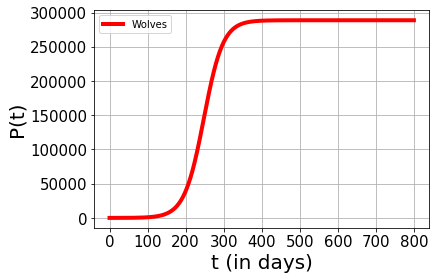
\includegraphics[scale=0.78]{Pictures/Wolves.png}
    \caption{Solution for $\frac{dP_w(t)}{dt} = R_wP_w(t)(1-\frac{P_w(t)}{M_w})$, where the wolves start at $20$.}
    \label{fig:Wolves}
\end{figure}
The Figure \ref{fig:Wolves} depicts that the model reaches an equilibrium around 288785. This can also be confirmed analytically. 
$$0=R_wP_w(t)(1-\frac{P_w(t)}{M_w})$$
$$R_wP_w(t)=0$$
$$1-\frac{P_w(t)}{M_w}=0$$
$$P_w(t)=M_w$$
$$P_w(t)=288785$$
Which means that the equilibrium solutions are 0 and 919996. We can find the extra deathrate due to lack of space with the following formula.
$$\alpha_w = a_w*\overline{W}$$
Where $\alpha_w$ is $b_w-d_w$, $a_w$ is the extra deathrate on top of the constant deathrate due to space limitations and $\overline{W}$ is the amount of wolves in the equilibrium situation, so $\overline{W}=288785$, so $a_w$ can be found by
$$a_w = \frac{\alpha_w}{\overline{W}}$$
Now we see that $a_w=1.3621735893484772*10^{-7}$. We find the extra birthrate due to the extra food available can be found by
$$\alpha_w + c_w*\overline{K}-a_w*\overline{W}=0$$
Here $c_w$ is the extra birthrate due to the extra food available, so $c_w$ can be found with
$$c_w=\frac{-\alpha+a_w*\overline{W}}{\overline{K}}$$
Thus can be found that $c_w=0$, so the differential equation becomes
$$\frac{dP_w(t)}{dt}=(b_w-d_w)*P_w*(1-\frac{1}{Mw}*P_w)$$
As grey wolves eat around 1.3607775 rabbit per day in optimal circumstances. The extra deathrate due to wolves eating rabbits can be found with
$$a_k*\overline{W}*\overline{K}=1.3607775*\overline{W}$$
This means that the extra deaths of rabbits due to being eaten by wolves is 
$$a_k=\frac{1.3607775}{\overline{K}}$$
So $a_k=1.0978*10^{-10}$. So the derivative equations we get are
$$\frac{dP_k}{dt}=(b_k-d_k)*P_k*(1-\frac{P_k}{M_k})-a_k*P_k*P_w$$
and 
$$\frac{dP_w}{dt}=(b_w-d_w)*P_w*(1-\frac{P_w}{M_f})$$
\begin{figure}[h!]
    \centering
    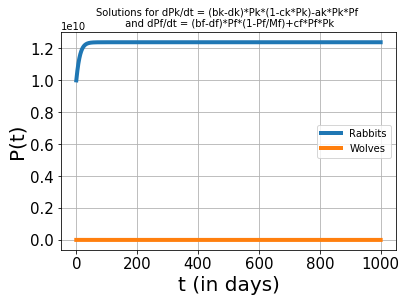
\includegraphics[scale=0.78]{Pictures/RabbitWolves.png}
    \caption{Solutions for $\frac{dP_k}{dt}=(b_k-d_k)*P_k*(1-\frac{P_k}{M_k})-a_k*P_k*P_f$ and $\frac{dP_w}{dt}=(b_w-d_w)*P_w*(1-\frac{P_w}{M_w})$, where the rabbits start at $1.0*10^{10}$ and the wolves at $288785$.}
    \label{fig:RabbitsWolves}
\end{figure}
As the Figure \ref{fig:RabbitsWolves} depicts, the amount of rabbits grow to its equilibrium of $1.23919001*10^{10}$ (from around 10000000000) and the wolves find their equilbrium around $288785$. In the graph is visible that wolves also don't do much to decimate the population of rabbits, due to the small number of wolves that can live on Australia and the fact that they don't eat enough rabbits to do much to their numbers. The code used for this model can be found in appendix \ref{WolfRabbitModel}.
%https://wolf.org/wolf-info/basic-wolf-info/wolf-faqs/#toggle-id-19
%https://wolfhaven.org/conservation/wolves/basic-facts-about-gray-wolves/
\section{Conclusion}
We find that introducing a natural predator to the rabbits won't work, as they do not eat enough rabbits per predator and need too much space. This means that Australia can not house enough predators to have an effect on the rabbit population.
\medskip
\bibliography{MyRef}
\appendix
\section{Code of the Fox-Rabbit model}\label{FoxRabbitModel}
\lstinputlisting[language=python]{KonijnenVossen.py}
\section{Code of the Wolf-Rabbit model}\label{WolfRabbitModel}
\lstinputlisting[language=python]{RabbitsWolves.py}
\end{document}
